\documentclass[10pt]{beamer}
\usetheme{PaloAlto}
\usecolortheme{seahorse}
\setbeamertemplate{navigation symbols}{}
\setbeamertemplate{caption}[numbered]
%general package
%\usepackage[utf8]{inputenc}
\usepackage{array}
\usepackage[english]{babel}
\usepackage{geometry}
\usepackage{tcolorbox}
\usepackage[export]{adjustbox}
\usepackage{graphicx}
\usepackage{xcolor}
\graphicspath{{../img}}
\hypersetup{
    colorlinks=true, 
    linkcolor=red,    % Internal links
    urlcolor=blue     % External links
}

%math package
\usepackage{amsmath}
\usepackage{amsfonts}
%\usepackage{amssymb}
%\usepackage{amsthm}
%\usepackage{slashed}
%\usepackage{tikz-cd}

%font package
%\usepackage{mathrsfs}
%\usepackage{bm}

%misc. package
\usepackage{enumitem}
\usepackage{animate}

\DeclareMathOperator{\xd}{\,d\!}
\DeclareMathOperator{\curl}{curl}
\DeclareMathOperator{\dive}{div}
\newcommand{\e}{{\rm e}}
\newcommand{\norm}[1]{\lVert#1\rVert}
\newcommand{\R}{\mathbb R}
\newcommand{\vF}{\mathbf F}
\newcommand{\vv}{\mathbf v}
\newcommand{\inpr}[1]{\left\langle#1\right\rangle}

\author[B.H.]{{\Large High School Algebra}\\\vspace{.5em} Instructor: Ben Huang}
\date{}
\title[Intro to Function]{Introduction to Functions}

%\institute[MU]{\vskip -2em
\includegraphics[width = 0.65\textwidth]{CityPoly.png}}
%\logo{
\includegraphics[width=.12\textwidth]{CityPolySmall.png}}

\begin{document}
\frame{\titlepage}

\section{why functions}
\begin{frame}
\frametitle{Why Functions?}
\begin{center}
Relations are everywhere.
\vspace{1em}

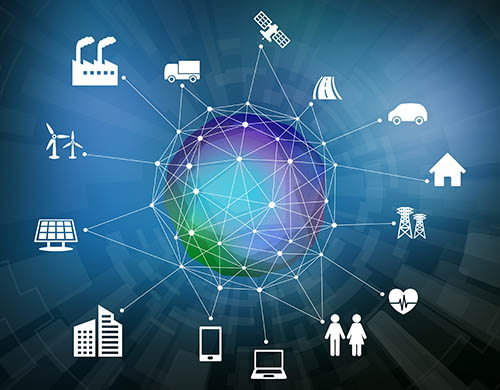
\includegraphics[width=0.7\textwidth]{IOT.jpg}
\vspace{1em}\pause

Mathematics is to study relations quantitatively.  
\end{center}

\end{frame}
\begin{frame}
\frametitle{Why Functions?}
\centering
{\Large Time - Position Relation}
\vspace{2em}

Input: time\hspace{3em}Output: position
\vspace{2em}

\begin{tabular}{cc}
\animategraphics[loop, autoplay, width=0.45\textwidth]{32}{projectile-}{000}{073}&\animategraphics[loop, autoplay, width=0.45\textwidth]{3}{parabola-}{000}{019}
\end{tabular}
\end{frame}

 \setbeamercolor{background canvas}{bg=black} 
\begin{frame}
\color{white}
\frametitle{Why Functions?}
\centering
{\Large Time - Position Relation}
\vspace{2em}

Input: time\hspace{3em}Output: position
\vspace{2em}

\begin{tabular}{cc}
\animategraphics[loop, autoplay, width=0.45\textwidth]{10}{planetary-}{000}{116}&\animategraphics[loop, autoplay, width=0.45\textwidth]{13}{solar-}{000}{104}
\end{tabular}
\end{frame}

 \setbeamercolor{background canvas}{bg=black} 
\begin{frame}
\color{white}
\frametitle{Why Functions?}
\centering
{\Large Neural Network - a fancy way to discover relations}
\vspace{2em}

Input: pixels\hspace{3em}Output: the recognized number
\vspace{2em}

\animategraphics[loop, autoplay, width=0.8\textwidth]{19}{neural-}{000}{120}
\end{frame}

 \setbeamercolor{background canvas}{bg=white} 
\begin{frame}
\frametitle{Why Functions?}
\centering
{\Large Event - Probability Relation - the endeavor to understand randomness}
\vspace{2em}

Input: event\hspace{3em}Output: probability
\vspace{2em}

\begin{tabular}{cc}
\animategraphics[loop, autoplay, width=0.45\textwidth]{1}{normal1-}{000}{004}&\animategraphics[loop, autoplay, width=0.45\textwidth]{1}{normal2-}{000}{003}
\end{tabular}
\end{frame}

\section{representations}
\begin{frame}
\frametitle{Function Representations}
\centering
\[
\parbox{10em}{input from the \underline{domain}}\longrightarrow\text{rule}\longrightarrow\parbox{10em}{{\bf unambiguous} output in the \underline{range}}
\]

\vspace{2em}

\animategraphics[loop, autoplay, width=\textwidth]{50}{function-}{000}{200}
\end{frame}

\section{exercises}
\begin{frame}
\frametitle{Exercises}
\centering
Time to get your hands dirty!
\vspace{2em}

\href{https://webwork.messiah.edu/webwork2/myTestCourse/Introduction_to_functions?effectiveUser=bhuang}{Exercises on WeBWork}
\vspace{2em}

\href{./Exercises-Intro-to-functions.pdf}{Exercises Offline Version}
\end{frame}
\end{document}